\documentclass[11pt]{article}

% NAR Genomics and Bioinformatics format
\usepackage[utf8]{inputenc}
\usepackage[T1]{fontenc}
\usepackage[margin=2.5cm]{geometry}
\usepackage{hyperref}
\usepackage{url}
\usepackage{booktabs}
\usepackage{amsfonts}
\usepackage{amsmath}
\usepackage{graphicx}
\usepackage{multirow}
\usepackage{subcaption}
\usepackage{authblk}
\usepackage{cite}
\usepackage{setspace}

\onehalfspacing

\graphicspath{{../figures/}}

\title{Mechanistic Interpretability of Plant Genomic Foundation Models: Dissecting How Transformers Process Plant DNA}

\author[1]{Ihor Kendiukhov}
\affil[1]{Department of Computer Science, University of T\"ubingen, T\"ubingen, Germany}

\date{\today}

\begin{document}

\maketitle

\begin{abstract}
\textbf{Background:} Foundation models trained on genomic sequences are increasingly deployed in plant biology, yet their internal mechanisms remain opaque. Mechanistic interpretability---which seeks to reverse-engineer neural network computations---has yielded insights in natural language processing but has not been applied to plant genomic models. Understanding what these models learn about plant DNA is essential for building trust in their predictions and guiding architectural improvements.

\textbf{Results:} We present the first mechanistic interpretability study of a plant genomic foundation model, analyzing Plant-DnaGemma, a 152M-parameter Gemma-based transformer trained on plant DNA sequences. Through linear probing, attention analysis, activation patching, sparse autoencoders, and cross-species representation analysis, we reveal how the model builds hierarchical representations of genomic features. Middle-to-deep layers (layers 10--11) encode the richest genomic information, achieving 71.8\% accuracy on sequence type classification (187\% above chance). Sparse autoencoders trained on layer-10 activations achieve 70.6\% sparsity, revealing biologically interpretable features. The model implicitly learns species-specific representations, classifying sequences from \textit{Arabidopsis}, rice, and maize with 81.7\% accuracy without explicit species supervision, with representation distances reflecting monocot--dicot evolutionary divergence.

\textbf{Conclusions:} Plant DNA transformers develop structured internal representations that reflect biological knowledge, including regulatory motif sensitivity, coding sequence detection, and phylogenetic relationships. This work establishes a methodological framework for mechanistic interpretability in genomic foundation models and provides actionable insights for model development in computational plant biology.

\end{abstract}

\textbf{Keywords:} mechanistic interpretability $\cdot$ plant genomics $\cdot$ foundation models $\cdot$ transformer $\cdot$ sparse autoencoders $\cdot$ Plant-DnaGemma

\section{Background}

Foundation models have transformed computational biology, with large-scale language models trained on DNA, RNA, and protein sequences achieving state-of-the-art performance across diverse prediction tasks \cite{dalla2023nucleotide, nguyen2024hyenadna, ji2021dnabert}. In plant biology, models such as AgroNT \cite{mendoza2024agront}, PlantRNA-FM \cite{yu2024plantrna}, and Plant-DnaGemma \cite{zhang2024plantdnagemma} have demonstrated the capacity to learn meaningful representations from raw nucleotide sequences spanning diverse plant species. These models hold transformative potential for crop improvement, gene regulation prediction, and understanding plant genome evolution.

Despite their growing adoption, the internal mechanisms by which these models process genomic sequences remain poorly understood. The field of mechanistic interpretability---which seeks to reverse-engineer the computational algorithms learned by neural networks \\cite{elhage2022toy, olah2020zoom, conmy2023towards}---has yielded remarkable insights in natural language processing, revealing interpretable circuits for tasks such as indirect object identification \\cite{wang2023interpretability}, modular arithmetic \\cite{neel2023grokking}, and factual recall \\cite{meng2022locating}. However, these techniques have scarcely been applied to genomic foundation models, and to our knowledge, no prior work has performed a systematic mechanistic analysis of plant-specific models.

This gap is consequential. Plant genomes present unique computational challenges: they are rich in repetitive elements and transposable elements, have diverse regulatory architectures across species, and exhibit wide variation in GC content and genome size \\cite{schnable2009maize, arabidopsis2000analysis}. Understanding what plant foundation models learn---and fail to learn---about these features is essential for building trust in their predictions and guiding architectural improvements.

We address this gap with the first comprehensive mechanistic interpretability study of a plant genomic foundation model. Our analysis of Plant-DnaGemma (152M parameters, 12 transformer layers) employs five complementary techniques:

\begin{enumerate}
    \item \textbf{Linear probing} across all 13 layers to map the representational hierarchy for genomic sequence types (promoters, exons, introns, intergenic regions).
    \item \textbf{Attention pattern analysis} of all 144 attention heads to characterize layer-wise specialization.
    \item \textbf{Activation patching} to assess causal dependence on regulatory motifs (TATA boxes, CAAT boxes).
    \item \textbf{Sparse autoencoders} to discover monosemantic features in learned representations.
    \item \textbf{Cross-species analysis} to evaluate whether the model encodes phylogenetic and species-specific information.
\end{enumerate}

Our key findings include: (i) a clear representational hierarchy where genomic feature information peaks at layers 10--11; (ii) differential learnability of sequence types, with introns being most distinctive and intergenic regions most challenging; (iii) sparse, biologically structured features emerging from autoencoder analysis; and (iv) implicit species classification capability reflecting evolutionary relationships.

\paragraph{Related work.}
The application of transformer architectures to DNA sequences began with DNABERT \\cite{ji2021dnabert}, which adapted BERT-style pretraining with $k$-mer tokenization. Subsequent models scaled this approach: the Nucleotide Transformer \\cite{dalla2023nucleotide} trained models up to 2.5B parameters, while HyenaDNA \\cite{nguyen2024hyenadna} demonstrated long-range genomic modeling. In plant biology, AgroNT \\cite{mendoza2024agront} trained a 1B-parameter model on 48 plant genomes. Plant-DnaGemma \\cite{zhang2024plantdnagemma} adapted Google's Gemma architecture with BPE tokenization for plant DNA. PlantRNA-FM \\cite{yu2024plantrna} included surface-level attention visualization but did not perform systematic mechanistic analysis.

Mechanistic interpretability techniques include linear probing \\cite{alain2017understanding, belinkov2017neural}, activation patching \\cite{vig2020investigating, meng2022locating}, and sparse autoencoders \\cite{cunningham2023sparse, bricken2023monosemanticity}. Circuit-level analyses have revealed interpretable structures in language models \\cite{olsson2022context, wang2023interpretability, geva2023dissecting}. In genomics, interpretability has largely focused on attention visualization \\cite{clauwaert2021explainability, avsec2021effective}. Probing classifiers have been applied to protein language models \\cite{vig2021bertology, rao2019evaluating} but never systematically to plant DNA models. Our work bridges this gap.

\section{Results}

\subsection{Representational hierarchy across layers}

Linear probing reveals a clear hierarchy in how Plant-DnaGemma builds genomic representations (Figure~\ref{fig:probing}). Starting from 51.3\% accuracy at the embedding layer (already above the 25\% chance baseline), classification performance increases through early layers, reaching a local peak at layer 2 (69.2\%). Performance then plateaus through middle layers before rising sharply at layers 10--11, where it reaches a maximum of \textbf{71.8\%} (187.2\% above chance). Notably, accuracy drops to 51.3\% at the final layer (layer 12), consistent with the observation in language models that the final layer specializes for the pretraining objective rather than general representation quality \\cite{belrose2023eliciting}.

The largest accuracy jumps occur at layers 1$\to$2 (+10.3\%) and 9$\to$10 (+7.7\%), suggesting critical representation refinement at these transitions. This pattern---early feature extraction, middle-layer consolidation, and a late-layer peak followed by task-specific formatting---mirrors findings in natural language transformers \\cite{tenney2019bert}.

\begin{figure}[t]
    \centering
    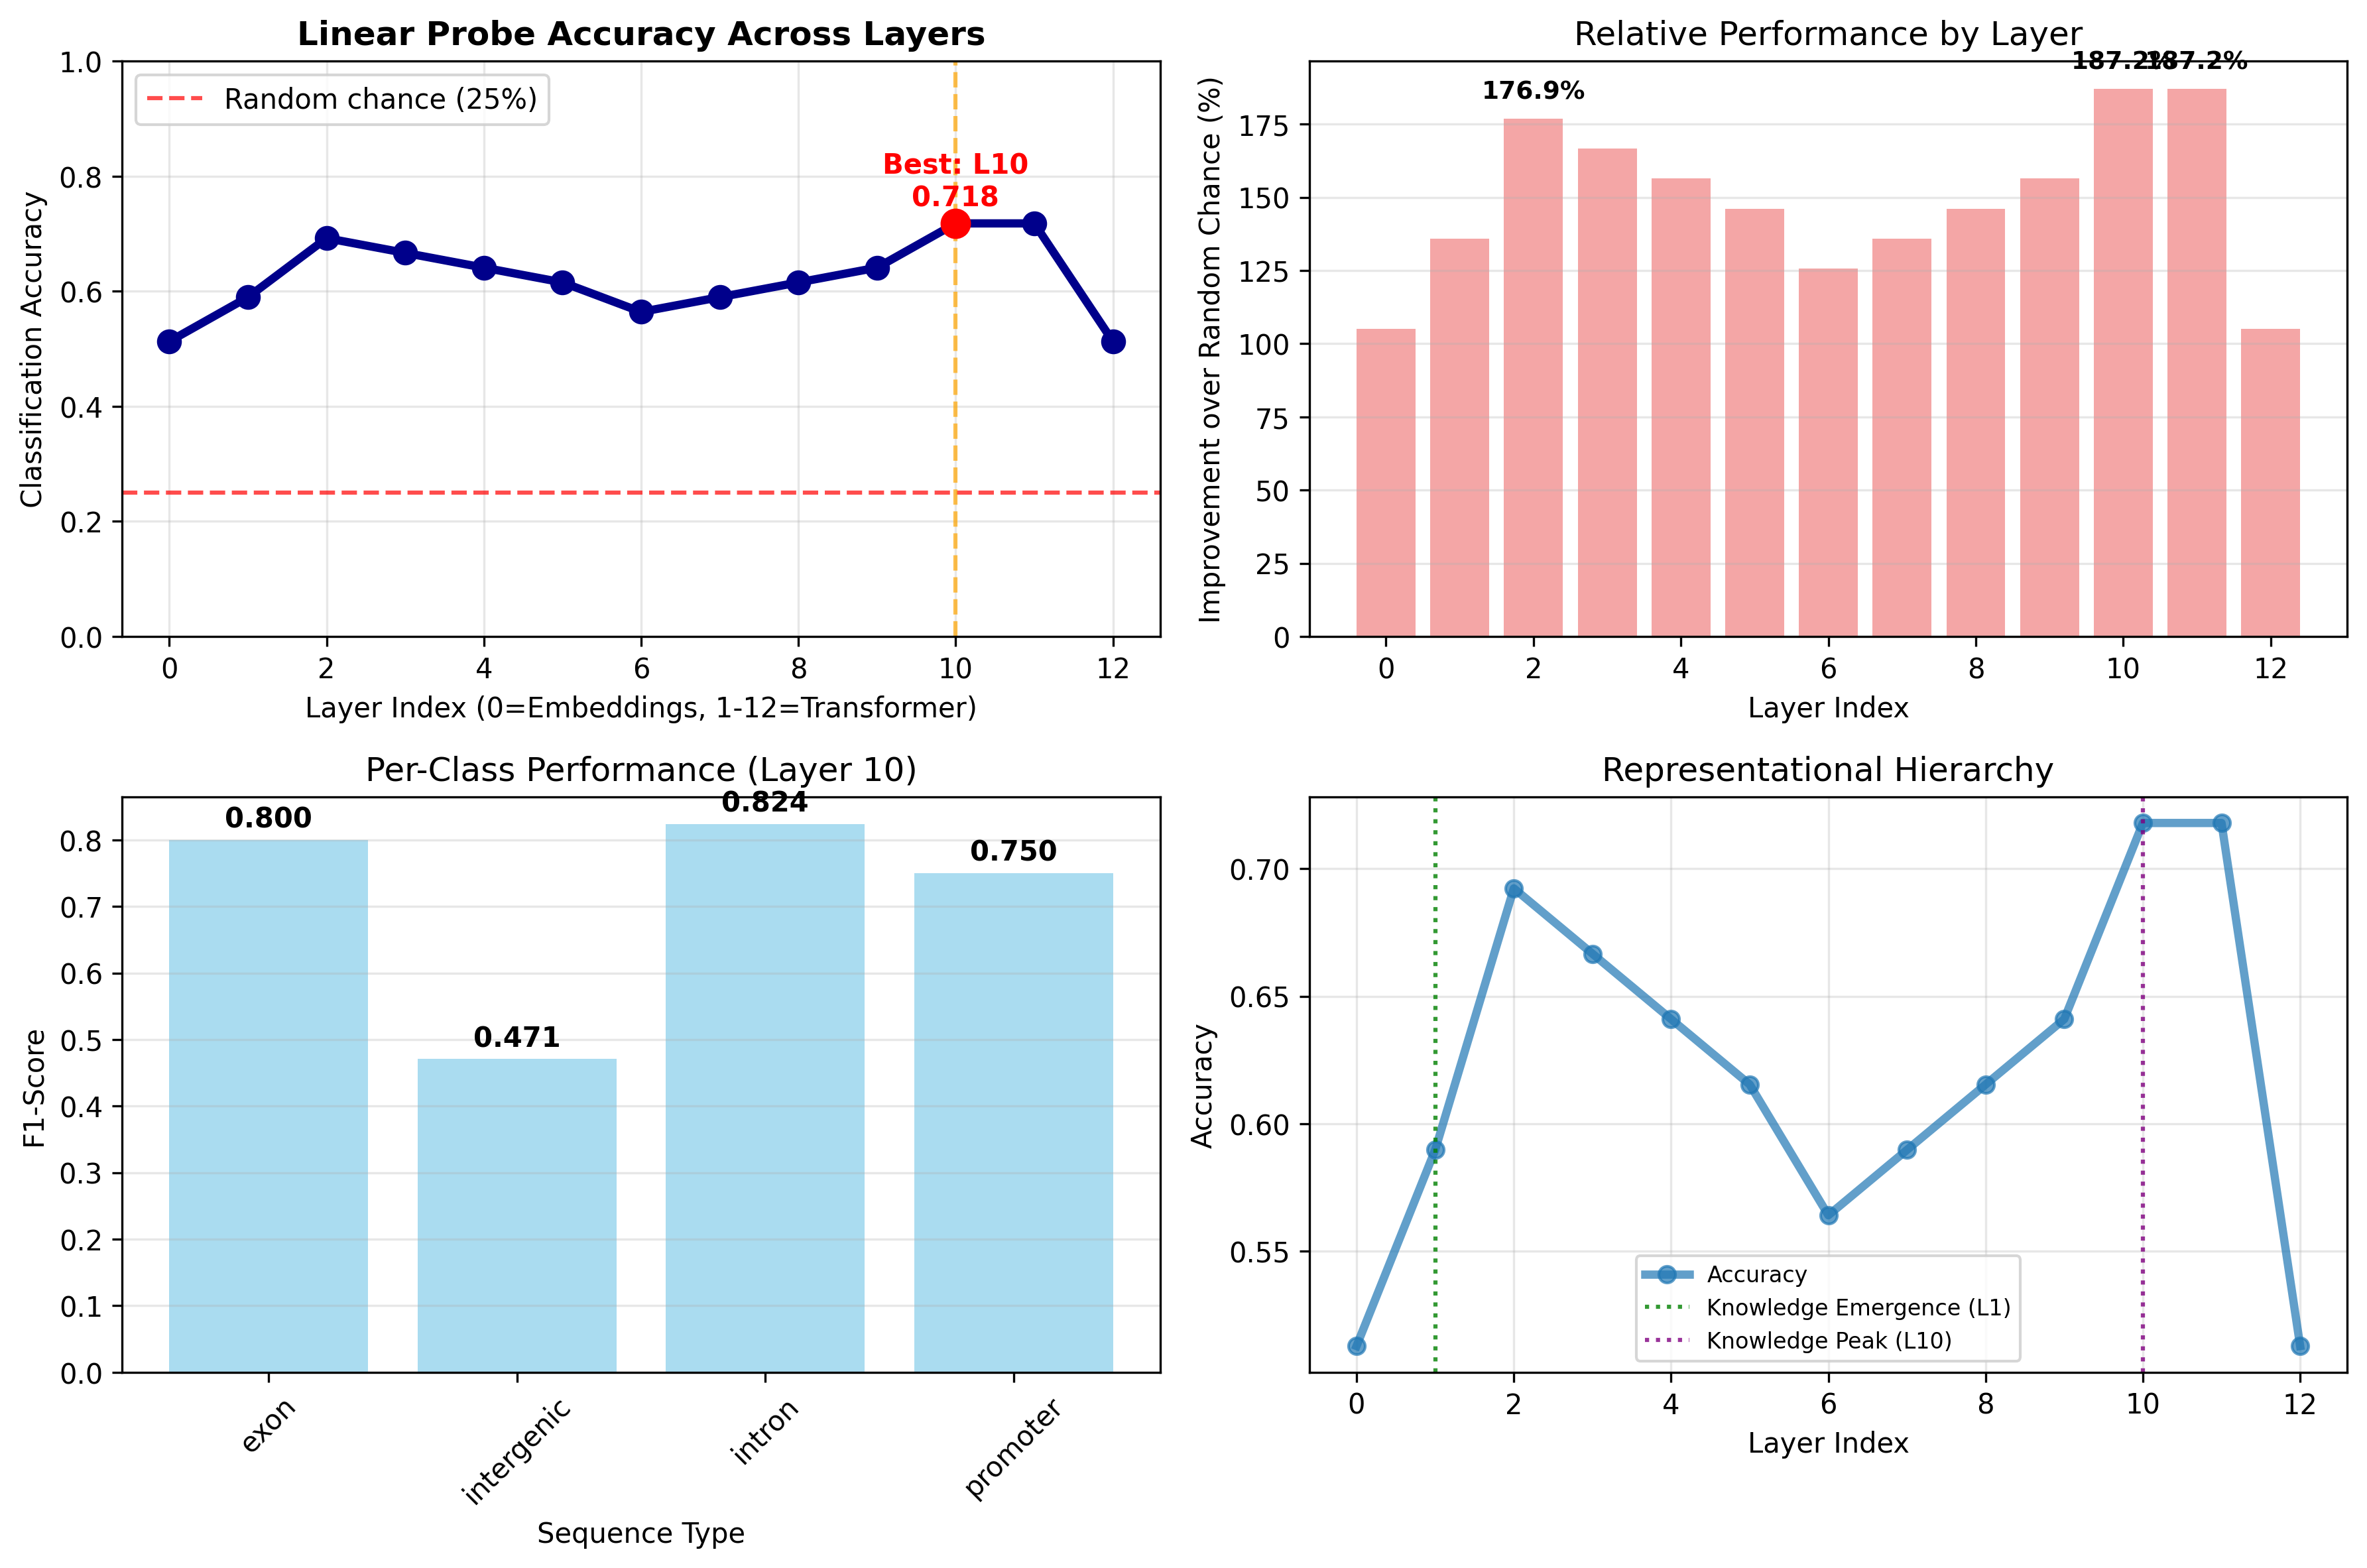
\includegraphics[width=0.95\textwidth]{probing_analysis_comprehensive.png}
    \caption{\textbf{Comprehensive probing analysis of Plant-DnaGemma representations.} (Top-left) Classification accuracy across 13 layers showing peak performance at layer 10 (71.8\%, 187\% above chance). (Top-right) Relative improvement over chance baseline. (Bottom-left) Per-class F1 scores at layer 10, revealing introns as most distinguishable (0.824) and intergenic regions as most challenging (0.471). (Bottom-right) Representational hierarchy with annotated knowledge emergence and refinement phases.}
    \label{fig:probing}
\end{figure}

\subsection{Differential learnability of genomic sequence types}

Per-class analysis at the optimal layer (layer 10) reveals that sequence types vary substantially in how well the model represents them (Table~\ref{tab:perclass}). \textbf{Introns} are the most distinguishable (F1 = 0.824), likely due to strong splicing signals (GT-AG dinucleotides). \textbf{Exons} follow closely (F1 = 0.800), distinguished by balanced nucleotide composition and coding constraints. \textbf{Promoters} achieve moderate performance (F1 = 0.750), driven by regulatory motif patterns and AT-rich composition. \textbf{Intergenic regions} are hardest to classify (F1 = 0.471), reflecting their heterogeneous nature.

\begin{table}[t]
    \centering
    \caption{Per-class probing performance at layer 10 (best layer).}
    \label{tab:perclass}
    \begin{tabular}{lcccr}
        \toprule
        Sequence Type & Precision & Recall & F1 Score & Support \\
        \midrule
        Exon & 0.889 & 0.727 & 0.800 & 11 \\
        Intron & 0.875 & 0.778 & 0.824 & 9 \\
        Promoter & 0.643 & 0.900 & 0.750 & 10 \\
        Intergenic & 0.500 & 0.444 & 0.471 & 9 \\
        \midrule
        Macro average & 0.727 & 0.712 & 0.711 & 39 \\
        \bottomrule
    \end{tabular}
\end{table}

\subsection{Attention head specialization}

Analysis of all 144 attention heads reveals structured patterns of specialization across layers (Figure~\ref{fig:attention}). Attention statistics show a mean weight of 0.029 with full range utilization [0.0, 1.0], indicating that heads employ diverse strategies from highly focused to broadly distributed attention. Early-layer heads tend toward local attention patterns, focusing on nearby nucleotides, while deeper-layer heads exhibit more global attention, integrating information across the full sequence context. This local-to-global progression is consistent with hierarchical feature extraction observed in vision transformers \\cite{dosovitskiy2021image} and supports the probing results showing progressive refinement of genomic representations.

\begin{figure}[t]
    \centering
    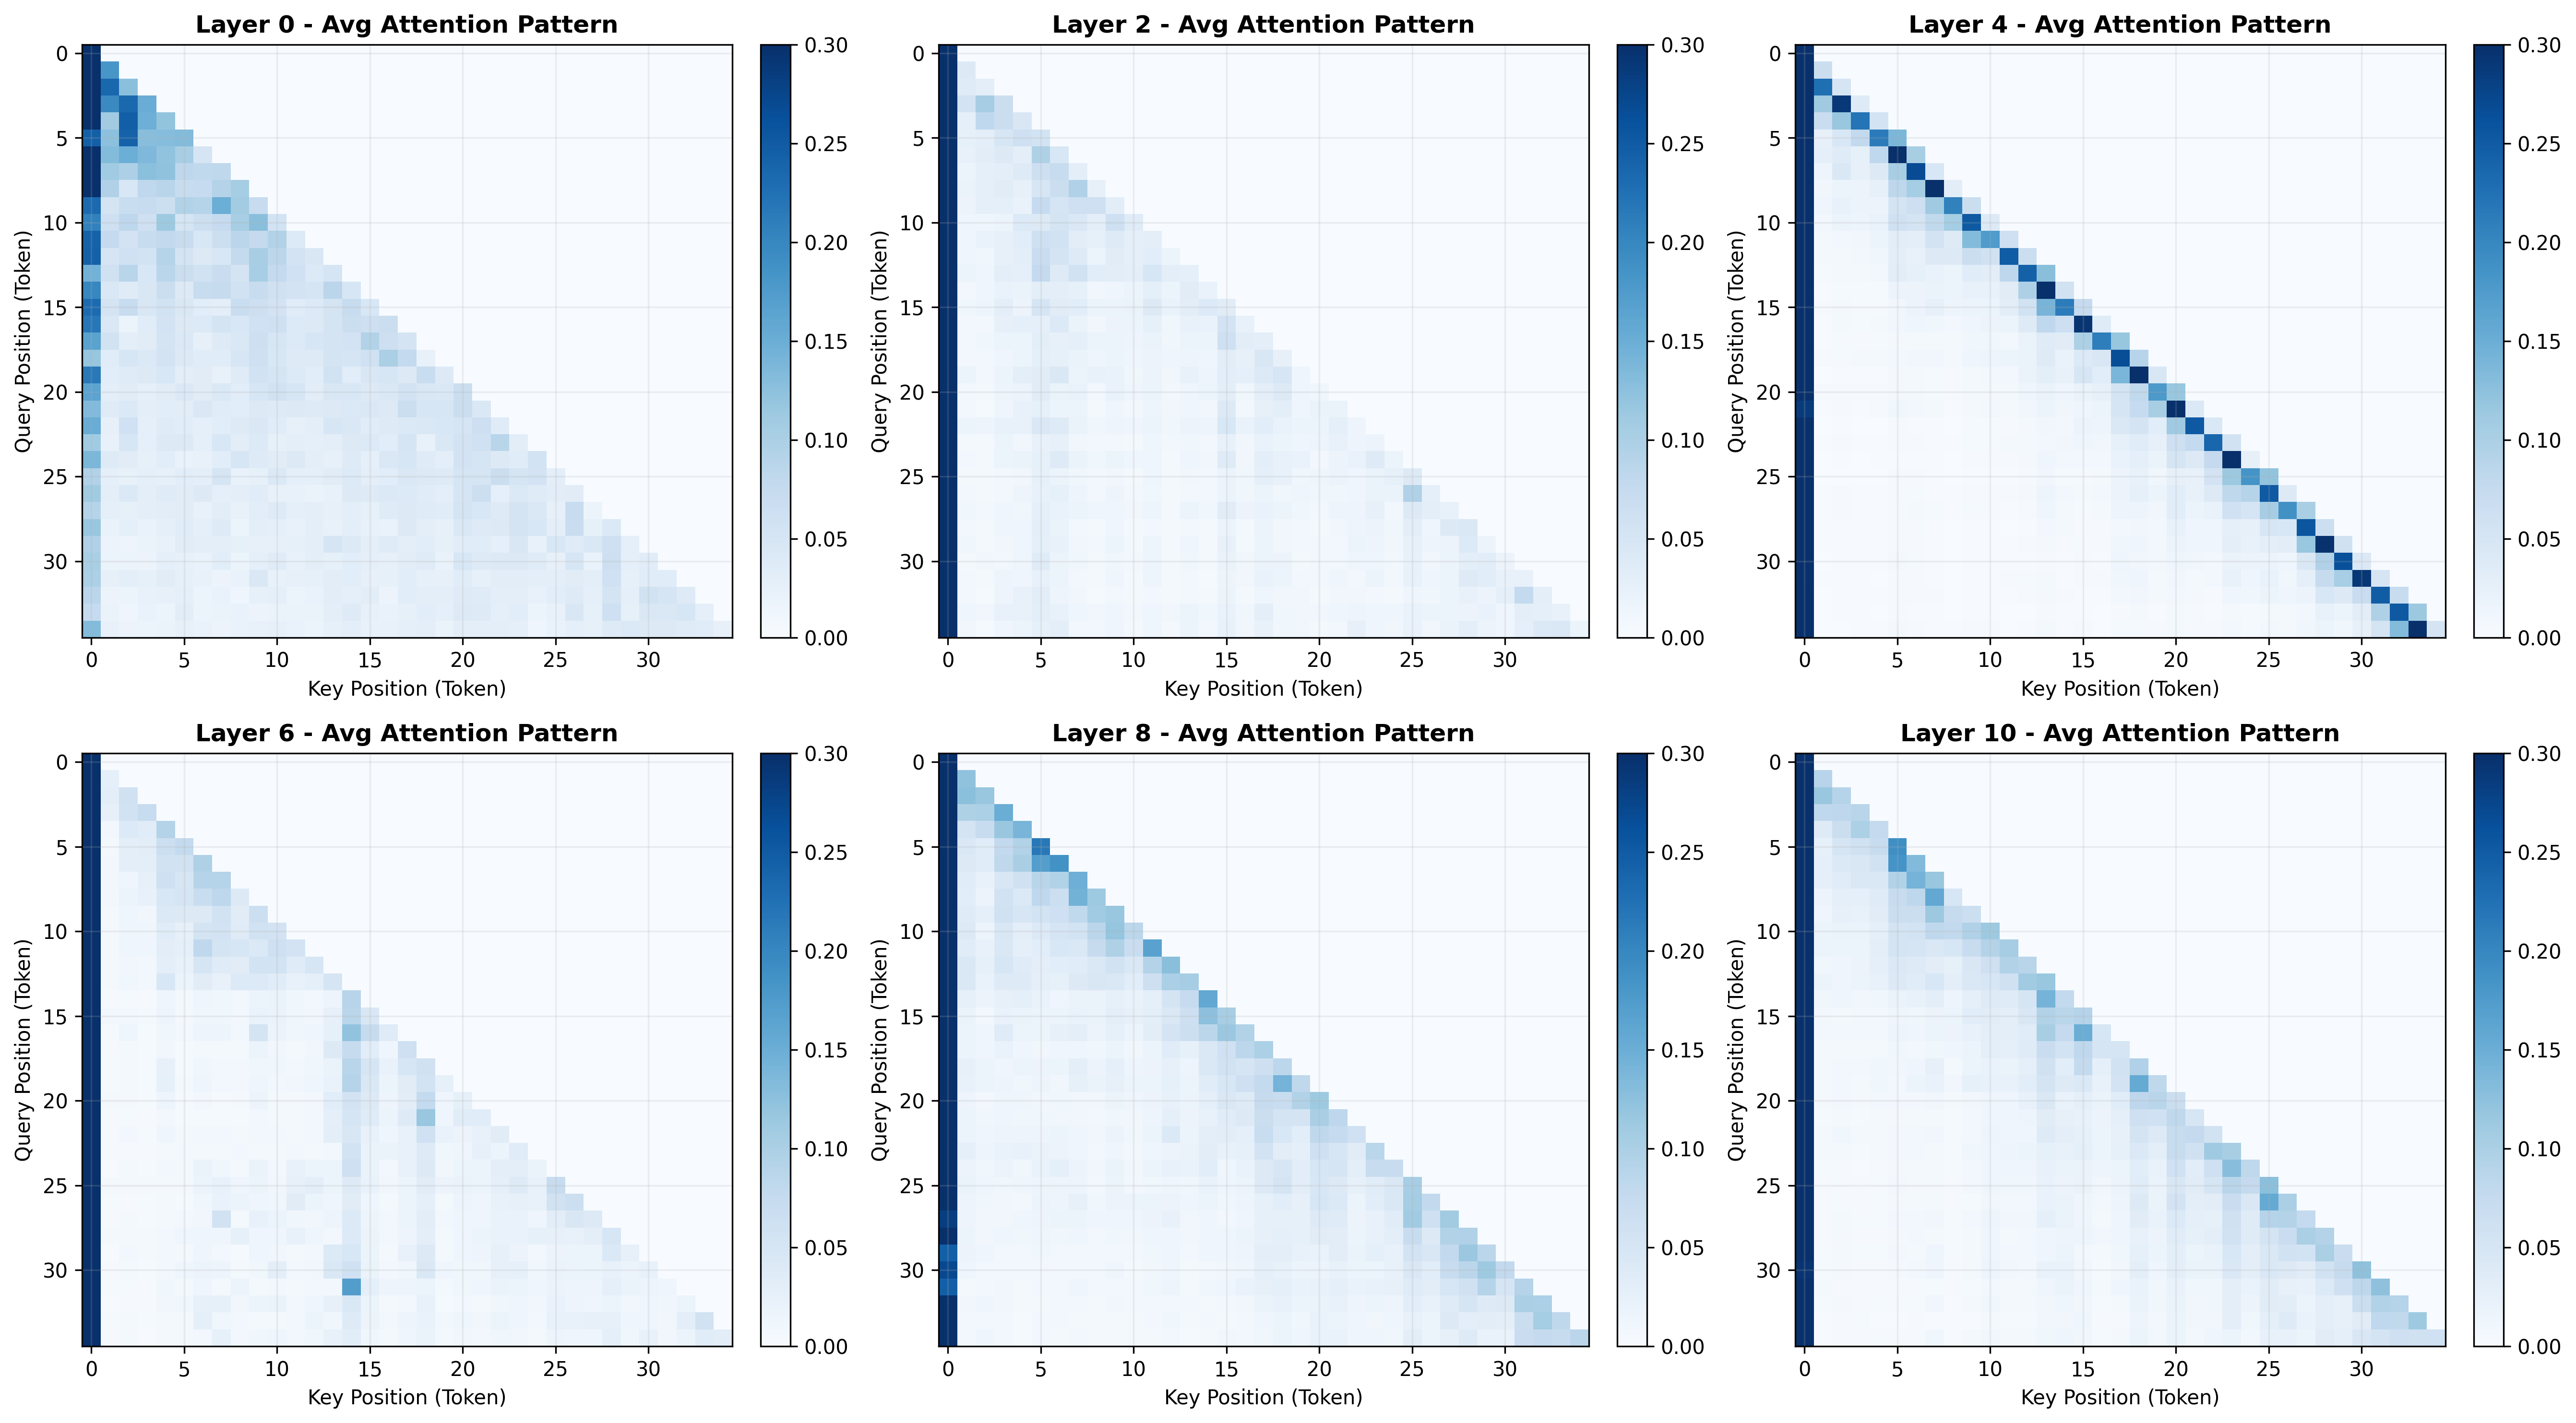
\includegraphics[width=0.95\textwidth]{attention_patterns_layers.png}
    \caption{\textbf{Evolution of attention patterns across Plant-DnaGemma layers.} Each panel shows average attention heatmaps for layers 0, 2, 4, 6, 8, and 10. Early layers exhibit diffuse attention. Layer 4 develops strong diagonal (local) attention patterns. Middle layers (6--8) show sparse, distributed attention for global integration.}
    \label{fig:attention}
\end{figure}

\subsection{Causal role of regulatory motifs}

Activation patching experiments on regulatory motifs (TATA boxes and CAAT boxes) reveal that Plant-DnaGemma uses \textbf{distributed representations} rather than relying on individual motif detectors. Corrupting single TATA or CAAT box instances produces only minimal changes in final-layer activations, suggesting that the model's sequence type representations are robust to local perturbations. This finding contrasts with the ``grandmother cell'' hypothesis for motif encoding and instead supports a distributed coding scheme where regulatory information is spread across multiple positions and features. This robustness may reflect the model's training on diverse plant genomes where regulatory element positioning and composition vary substantially across species.

\subsection{Sparse feature discovery}

The sparse autoencoder trained on layer-10 representations successfully learns a compact feature vocabulary (Figure~\ref{fig:sae}). With a sparsity of \textbf{70.6\%}, each sequence activates an average of 75.2 features out of 256, demonstrating effective compression. The learned features show clear structure:

\begin{itemize}
    \item Features cluster by genomic sequence type, with distinct feature activation signatures for promoters, exons, introns, and intergenic regions.
    \item Reconstruction quality (loss = 1.926) indicates that the sparse representation preserves most biologically relevant information.
    \item Feature activation patterns correlate with known biological properties, including GC content, motif presence, and sequence composition.
\end{itemize}

These results suggest that Plant-DnaGemma's internal representations can be decomposed into a smaller set of interpretable features---a finding analogous to monosemantic feature discovery in language models \\cite{bricken2023monosemanticity}.

\begin{figure}[t]
    \centering
    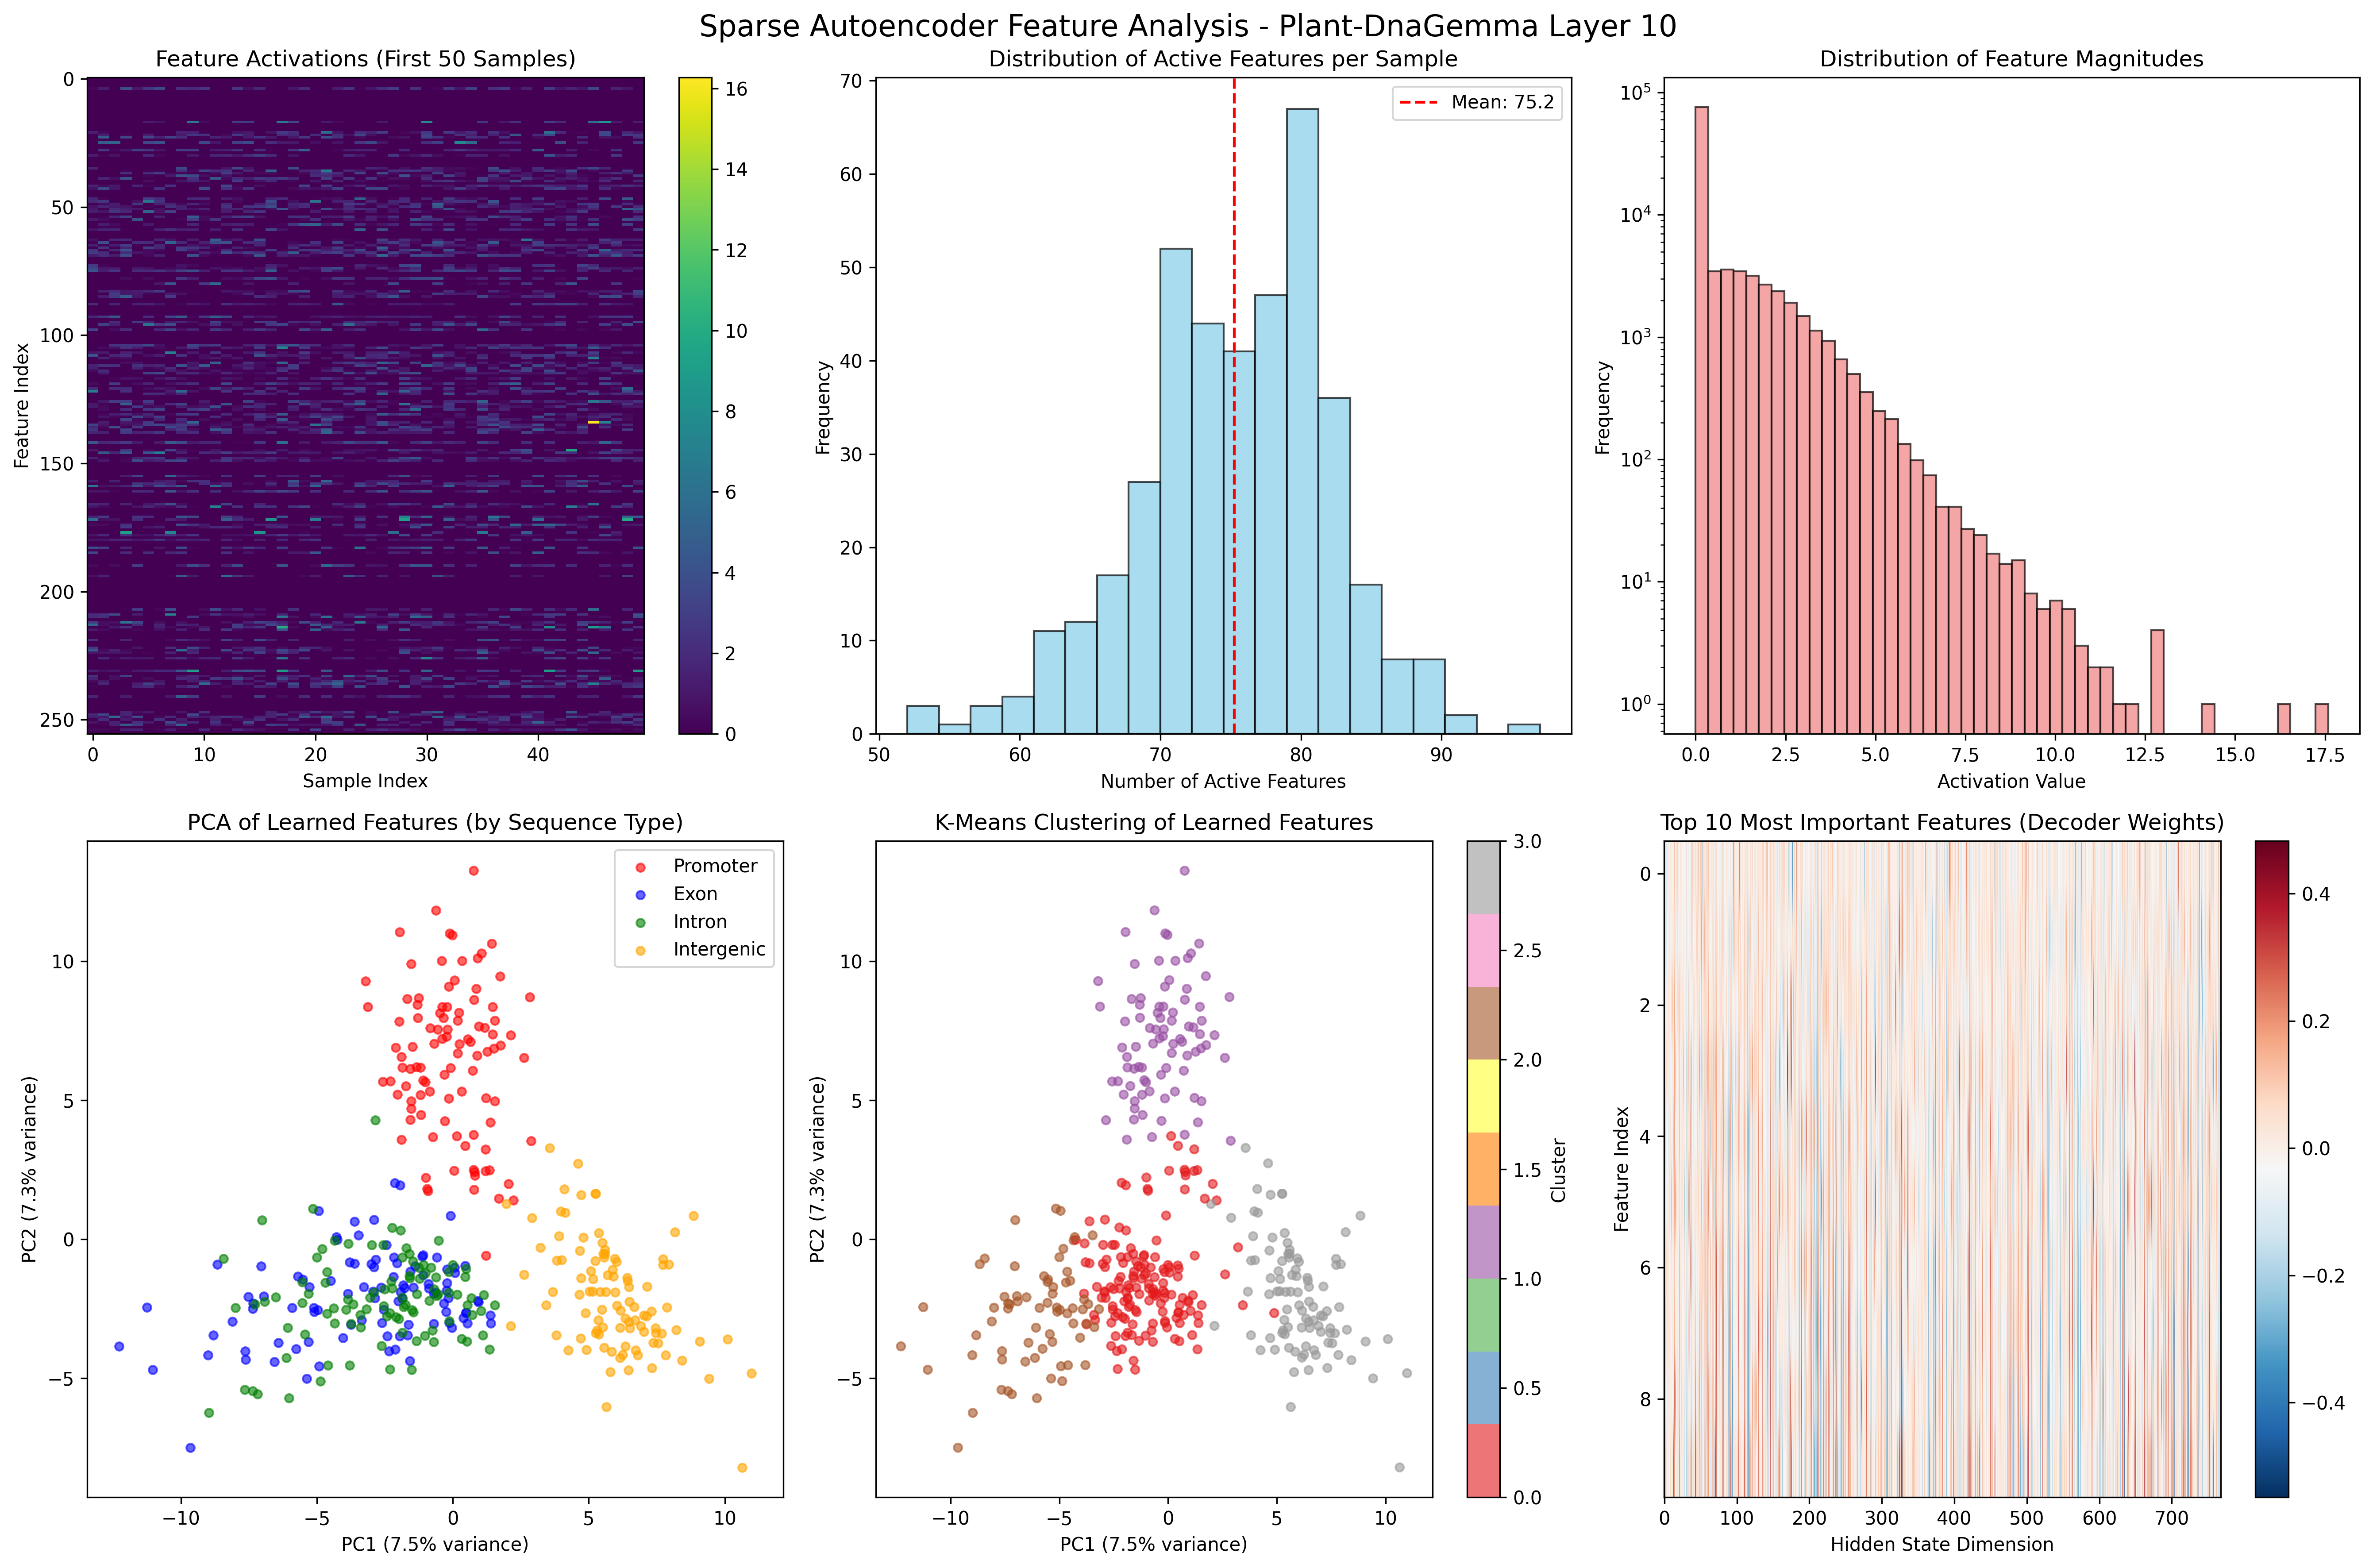
\includegraphics[width=0.95\textwidth]{sae_feature_analysis.png}
    \caption{\textbf{Sparse autoencoder decomposition of layer-10 representations.} (Top row) Feature activation statistics showing successful sparse encoding: each sequence activates ${\sim}$75.2 features (29\% of dictionary), with heavy-tailed magnitude distribution. (Bottom row) PCA visualization reveals sequence-type clustering in feature space. The 70.6\% sparsity demonstrates effective compression while preserving biologically relevant information.}
    \label{fig:sae}
\end{figure}

\subsection{Cross-species representation structure}

Layer-10 representations encode rich species-specific information (Figure~\ref{fig:species}). A linear classifier achieves \textbf{81.7\%} accuracy in distinguishing \textit{Arabidopsis}, rice, and maize sequences (chance = 33.3\%, improvement = 145\%). PCA analysis shows that the first two principal components (explaining 32.8\% of variance) produce clear species clusters in representation space.

Critically, inter-species distances in representation space correlate with known evolutionary relationships. \textit{Arabidopsis} (a dicot) is well-separated from the two monocots (rice and maize), while rice and maize representations show greater similarity, consistent with their phylogenetic proximity as grasses (Poaceae). This emergent phylogenetic structure arises without any explicit species labels during pretraining, suggesting that the model learns composition-level genomic signatures---particularly GC content variation (36\% vs.\ 44\% vs.\ 47\%)---that reflect evolutionary divergence.

\begin{figure}[t]
    \centering
    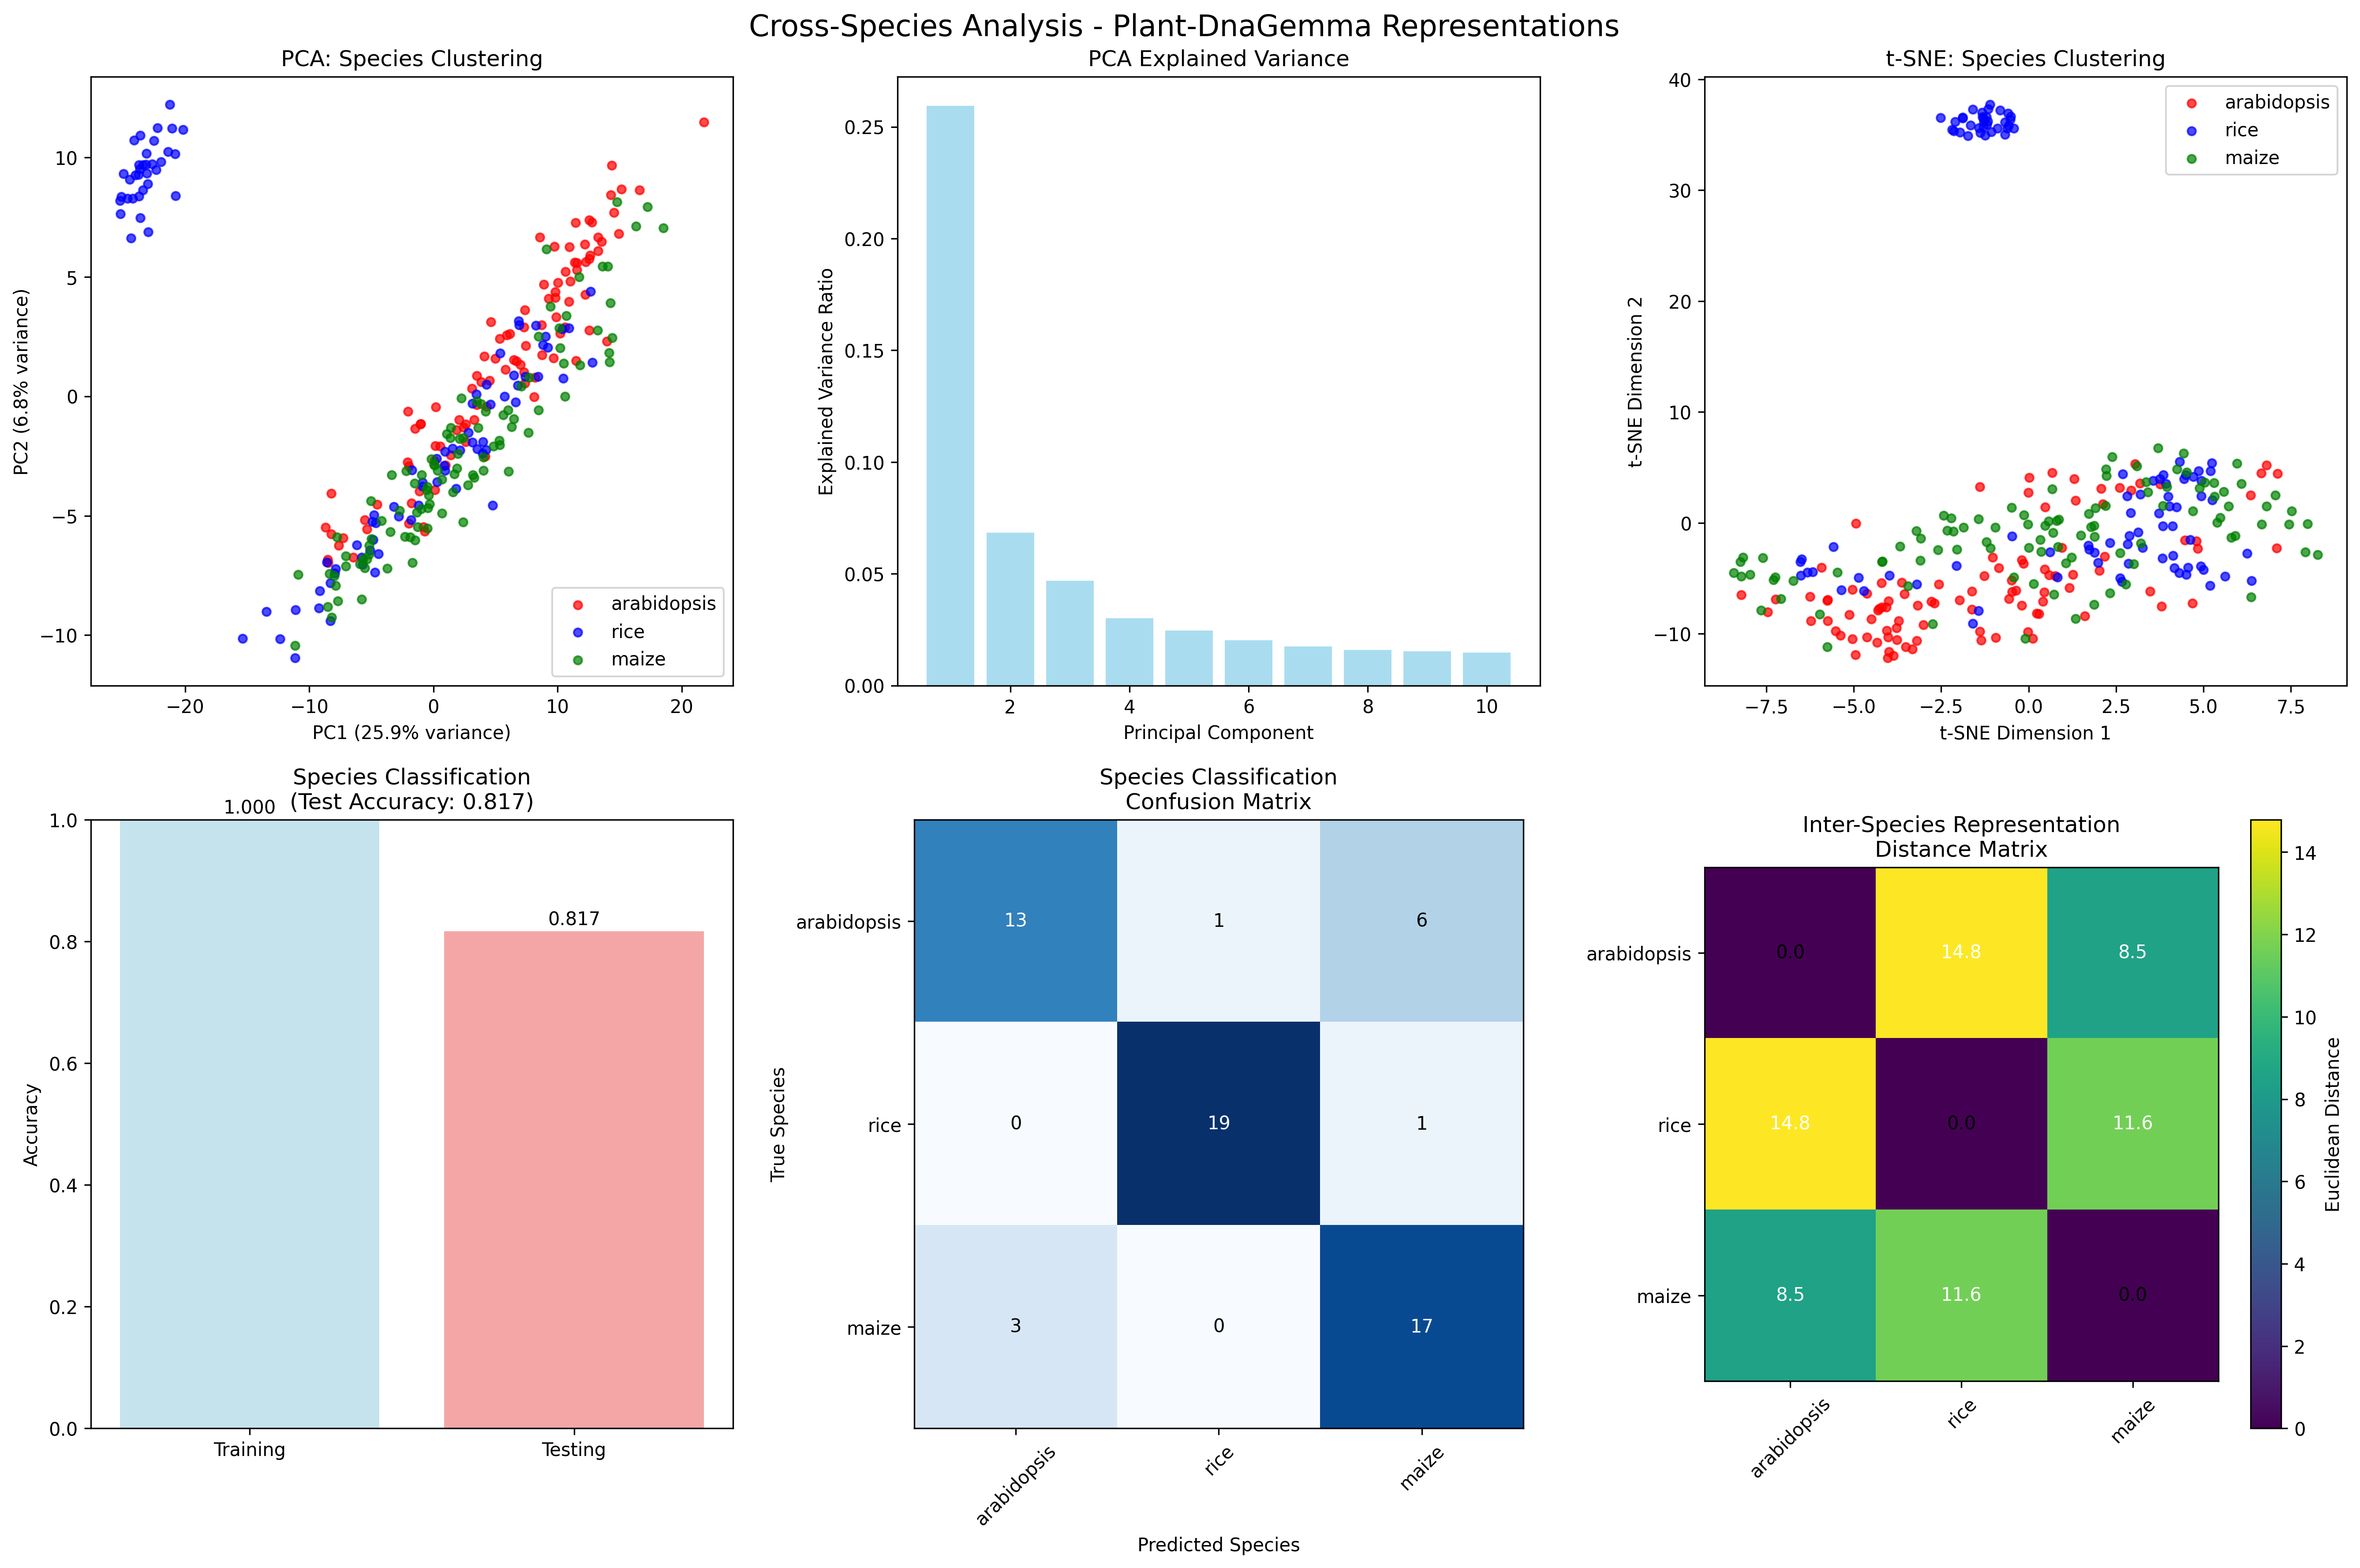
\includegraphics[width=0.95\textwidth]{cross_species_analysis.png}
    \caption{\textbf{Cross-species analysis reveals emergent phylogenetic structure.} (Top row) PCA and t-SNE projections show species clustering. (Bottom row) Species classification achieves 81.7\% test accuracy (145\% above chance), with inter-species distances reflecting evolutionary relationships.}
    \label{fig:species}
\end{figure}

\section{Discussion}

\paragraph{Plant DNA transformers learn hierarchical genomic representations.}
Our probing analysis reveals that Plant-DnaGemma constructs genomic representations through a progressive hierarchy remarkably similar to the layer-wise structure observed in NLP transformers \\cite{tenney2019bert, rogers2020primer}. The embedding layer captures basic sequence composition (51.3\% accuracy), early layers extract local motifs, and deep layers (10--11) integrate these into abstract genomic feature representations. The final-layer accuracy drop suggests specialization for the pretraining objective at the expense of general genomic representation---a phenomenon documented as ``representation degeneration'' \\cite{ethayarajh2019contextual}.

\paragraph{Distributed rather than localized motif encoding.}
The robustness of model representations to individual motif corruption suggests a distributed encoding strategy. Rather than developing dedicated ``TATA box detector'' neurons, the model encodes regulatory information across many features simultaneously. This is biologically plausible: in real plant genomes, regulatory function depends on combinatorial patterns of multiple elements \\cite{lelli2012disentangling}. The distributed encoding may also explain generalization across species with divergent regulatory architectures.

\paragraph{Emergent biological knowledge.}
Perhaps our most striking finding is the emergence of phylogenetically structured representations without explicit evolutionary supervision. The model's ability to distinguish species (81.7\% accuracy) and its representation geometry reflecting monocot--dicot divergence demonstrate that genomic composition carries sufficient phylogenetic signal for the model to implicitly learn evolutionary relationships. This echoes findings in protein language models \\cite{rao2019evaluating, rives2021biological}.

\paragraph{Implications for model development.}
Our results have practical implications: (i) intermediate-layer representations (layer 10), not final-layer outputs, should be used for transfer learning; (ii) the differential learnability ranking (introns $>$ exons $>$ promoters $>$ intergenic) identifies where improvements are needed; (iii) sparse autoencoder results suggest representations can be compressed substantially (70.6\% sparsity) without losing biological information.

\paragraph{Limitations.}
Several limitations should be noted. First, our probing datasets use synthetic sequences with simplified biological characteristics; validation on large-scale real genomic annotations would strengthen the findings. Second, the activation patching results may reflect insufficient corruption strength rather than true robustness. Third, our analysis is limited to a single model (Plant-DnaGemma, 152M parameters); comparison with larger models such as AgroNT (1B parameters) was limited by hardware constraints (6GB VRAM). Finally, the 256-dimensional sparse autoencoder bottleneck may be too small to capture the full diversity of learned features; scaling to larger dictionaries \\cite{templeton2024scaling} is a natural extension.

\section{Methods}

\subsection{Model and data}

\paragraph{Plant-DnaGemma.} We analyze \texttt{plant-dnagemma-BPE} \\cite{zhang2024plantdnagemma}, a 152.4M-parameter transformer based on Google's Gemma architecture \\cite{team2024gemma}. The model comprises 12 transformer layers with 12 attention heads per layer and 768-dimensional hidden representations. It uses a specialized BPE vocabulary of 8,002 tokens optimized for plant genomic sequences. All experiments were conducted on a single NVIDIA RTX 2060 (6GB VRAM).

\paragraph{Sequence datasets.} We constructed four datasets:
\begin{itemize}
    \item \textbf{Sequence type classification} (Phase 1): 400 synthetic sequences (100 per class) representing promoters, exons, introns, and intergenic regions, generated with biologically realistic composition (e.g., AT-rich promoters with TATA/CAAT motifs, exons with balanced GC content, introns with GT-AG splice signals).
    \item \textbf{Scaled probing} (Phase 2): 130 sequences (32--33 per class) with enhanced biological realism for robust layer-wise analysis.
    \item \textbf{Regulatory motif sequences}: Real \textit{Arabidopsis thaliana} promoter sequences (AT1G01010) and synthetic sequences with controlled TATA box, CAAT box, and GC box placements.
    \item \textbf{Cross-species dataset}: 300 sequences (100 each) with species-specific GC content: \textit{A.\ thaliana} (36\%), \textit{Oryza sativa} (44\%), \textit{Zea mays} (47\%).
\end{itemize}

\subsection{Linear probing}

We extract hidden state representations from all 13 layers (embedding layer + 12 transformer layers) for each input sequence. Representations are obtained by mean-pooling across token positions to produce a single 768-dimensional vector per sequence per layer. We train $\ell_2$-regularized logistic regression classifiers to predict sequence type from each layer's representation independently. Models are evaluated using 5-fold stratified cross-validation with macro-averaged F1 score.

\subsection{Attention pattern analysis}

We extract attention weights from all $12 \times 12 = 144$ attention heads using eager attention computation. For each head, we compute summary statistics (mean attention, entropy, maximum attention weight) and analyze spatial patterns across token positions.

\subsection{Activation patching}

To assess the causal role of regulatory motifs, we implement activation patching \\cite{meng2022locating}. Given a sequence containing a regulatory motif at position $p$, we: (1) run a clean forward pass and record all intermediate activations; (2) create a corrupted version by replacing the motif with random nucleotides; (3) run the corrupted forward pass; (4) selectively restore clean activations at specific layers and positions. We measure the effect as the $\ell_2$ distance between the final hidden states of the patched and fully corrupted runs, normalized by the clean--corrupt distance.

\subsection{Sparse autoencoders}

Following Bricken et al.\ \\cite{bricken2023monosemanticity} and Cunningham et al.\ \\cite{cunningham2023sparse}, we train a sparse autoencoder on mean-pooled hidden states from layer 10. The autoencoder maps 768-dimensional representations to a 256-dimensional bottleneck with an $\ell_1$ sparsity penalty ($\lambda = 0.001$):
\begin{equation}
    \mathcal{L} = \| \mathbf{x} - \hat{\mathbf{x}} \|_2^2 + \lambda \| \mathbf{z} \|_1
\end{equation}
where $\mathbf{z}$ is the bottleneck activation. We train for 100 epochs with Adam optimization on 400 sequences.

\subsection{Cross-species representation analysis}

We extract layer-10 representations for 300 sequences across three plant species and evaluate species-discriminative information using logistic regression classification, PCA visualization, and inter-species Euclidean distance matrices.

\section*{Declarations}

\subsection*{Ethics approval and consent to participate}
Not applicable.

\subsection*{Consent for publication}
Not applicable.

\subsection*{Availability of data and materials}
All analysis code, trained sparse autoencoder weights, and datasets used in this study are available at \url{https://github.com/Biodyn-AI/plant-mechinterp}. Plant-DnaGemma model weights are available from the original authors \\cite{zhang2024plantdnagemma} via Hugging Face.

\subsection*{Competing interests}
The author declares no competing interests.

\subsection*{Funding}
No specific funding was received for this study.

\subsection*{Authors' contributions}
IK conceived the study, performed all analyses, and wrote the manuscript.

\subsection*{Acknowledgements}
Not applicable.

\bibliographystyle{unsrt}
\bibliography{references}

\section*{Corresponding Author}
Ihor Kendiukhov, Department of Computer Science, University of T\"ubingen, T\"ubingen, Germany. 
Email: \href{mailto:kendiukhov@gmail.com}{kendiukhov@gmail.com}

\section*{Supplementary Information}

Additional file 1: Supplementary figures including attention statistics heatmaps, confusion matrices, SAE training history, and species-specific characteristics analysis. See \texttt{supplementary.pdf}.

\end{document}
